\documentclass[final,hyperref={pdfpagelabels=false}]{beamer}

\usepackage{graphics, subfigure}
\usepackage{color}
\usepackage[portuguese]{babel}
\usepackage[utf8]{inputenc}
\usepackage[orientation=portrait,size=a0,scale=1.4]{beamerposter}
\usepackage{fp}% http://ctan.org/pkg/fp
\usepackage{wrapfig} % wrap text around figures
\usepackage{calc} % easy adding dimensions
\usepackage[export]{adjustbox} % left, right-align includegraphics
\usepackage{caption}
\usepackage{amsmath}
\newlength{\columnheight}
\setlength{\columnheight}{98cm}
\def\marginwidthratio{0.08}
\FPeval{\contentwidthratio}{1-\marginwidthratio}
\FPeval{\tightcontentwidthratio}{1-(\marginwidthratio / 2)}
\def\insidecolumnsinter{0.05}

\graphicspath{{figures/}}
\newlength{\insidecolumnwidth}%
\newlength{\intercolumnwidth}%
\newlength{\titleheight}%
% Colors %%%%%%%%%%%%%%%%%%%%%%%%%%%%%%%%%%%%%%%%%%%%%%%%%%%%%%%%%%%%%%%%%%%%%

\definecolor{green_butantan}{RGB}{0,112,60}
\definecolor{c_purple}{RGB}{56,3,52}
\definecolor{c_blue}{RGB}{41,68,107}
\definecolor{alert_blue}{RGB}{70, 70, 255}
\definecolor{c_green}{RGB}{87,184,9}
\definecolor{green2}{RGB}{76,196,93}
\definecolor{green3}{RGB}{76,173,138}
\definecolor{turquoise}{RGB}{39,94,102}
\definecolor{c_orange}{RGB}{255,149,28}
\setbeamertemplate{navigation symbols}{}  % no navigation on a poster
\setbeamercolor*{block title}{fg=green_butantan!80,bg=white}
\setbeamerfont{footline}{size=\large}
%\setbeamerfont{block title}{size=\large,series=\bf}
\setbeamerfont{block title}{size={\fontsize{64}{24}}, series=\bfseries}
\setbeamerfont{title}{size={\fontsize{83}{10}}}
\setbeamerfont{author font}{size={\fontsize{56}{10}}}
\setbeamerfont{supervisor font}{size={\fontsize{50}{10}}}


% Itemize %%%%%%%%%%%%%%%%%%%%%%%%%%%%%%%%%%%%%%%%%%%%%%%%%%%%%%%%%%%%%%%%%%%%
\setbeamertemplate{itemize item}{\color{green_butantan}{\textbf{$\bullet$}~}\color{black!50}}
\setbeamertemplate{itemize/enumerate body begin}{\color{black!80}}
\setbeamertemplate{itemize subitem}{\color{green_butantan}{\textbf{\diamond}~}}
\setbeamertemplate{caption}[numbered]
\setbeamercolor{caption}{fg=black!80}
\setbeamercolor{caption name}{fg=green2}
\setbeamercolor*{enumerate item}{fg=green_butantan}
\setbeamercolor*{enumerate subitem}{fg=green_butantan}
\setbeamercolor*{enumerate subsubitem}{fg=green_butantan}
\setbeamerfont{enumerate item}{series=\bf}
\setbeamercolor*{background canvas}{bg=white}



\newcommand{\leftcolumn}[1]{%
\begin{column}{.49\textwidth}%        
\begin{minipage}[T]{\textwidth}%
\parbox[t][\columnheight]{\textwidth}{#1}%
\end{minipage}%
\end{column}%
}
\newcommand{\rightcolumn}[1]{%
\begin{column}{.49\textwidth}%        
\begin{minipage}[T]{\textwidth}%
\parbox[t][\columnheight]{\textwidth}{#1}%
\end{minipage}%
\end{column}%
}

\newcommand{\customparagraph}[2]{%
\parbox[t][]{\contentwidthratio\textwidth}{%
%\hspace*{2cm}%
#2}%
\vspace*{#1}%
~\\%
}
\newcommand{\paragraph}[1]{%
\parbox[t][]{\contentwidthratio\textwidth}{%
%\hspace*{2cm}%
#1}%
\vspace*{2cm}%
~\\%
}

\newcommand{\tightparagraph}[1]{%
\vspace*{-.5cm}\parbox[t][]{\textwidth}{%
%\hspace*{2cm}%
#1}%
~\\%
}

\newcommand{\leftfigparagraph}[4]{%
\parbox[t][]{\contentwidthratio\textwidth}{%
\setlength\intextsep{0pt}%
\begin{wrapfigure}[#3]{L}{#2cm+1cm}%
\includegraphics[width=#2cm,left]{#1}%
\end{wrapfigure}%
%\hspace*{2cm}%
#4}%
\vspace*{2cm}%
~\\%
}

\newcommand{\rightfigparagraph}[4]{%
\parbox[t][]{\contentwidthratio\textwidth}{%
\setlength\intextsep{0pt}%
\begin{wrapfigure}[#3]{R}{#2cm+1cm}%
\includegraphics[width=#2cm,right]{#1}%
\end{wrapfigure}%
%\hspace*{2cm}%
#4}%
\vspace*{2cm}%
~\\%
}


\newcommand{\myimage}[2]{%
\scalebox{#2}{\includegraphics{#1}}%
~\\%
}

\newcommand{\mycenteredimage}[2]{%
\begin{center}%
\scalebox{#2}{\includegraphics{#1}}%
\end{center}%
}

\newcommand{\insidecolumns}[4]{%
\FPeval{\insidecolumnsnoncontent}{\marginwidthratio + \insidecolumnsinter}
\FPeval{\insidecolumnscontent}{1 - \insidecolumnsnoncontent}
\setlength{\insidecolumnwidth}{\insidecolumnscontent\textwidth}%
\setlength{\intercolumnwidth}{\marginwidthratio\textwidth}%
\vspace{-2cm}%
\begin{columns}[t,onlytextwidth]%
%\vrule{}%
\begin{column}{.5\intercolumnwidth}~\end{column}%
%\vrule{}%
\begin{column}{#1\insidecolumnwidth}%
\begin{flushleft}%
#3~%
\end{flushleft}%
\end{column}%
%\vrule{}%
\begin{column}{\insidecolumnsinter\textwidth}~\end{column}%
%\vrule{}%
\begin{column}{#2\insidecolumnwidth}%
\begin{flushright}%
#4~%
\end{flushright}%
\end{column}%
%\vrule{}%
\begin{column}{.5\intercolumnwidth}~\end{column}%
%\vrule{}%
\end{columns}%
\vspace*{2cm}%
}

\newcommand{\myitemize}[1]{%
\vspace*{-2cm}%
\hspace*{1cm}\parbox[t][]{0.9\textwidth}{%
\begin{itemize}%
#1%
\end{itemize}%
}%
\vspace*{3cm}%
}

\newcommand{\myenumerate}[1]{%
\vspace*{-2cm}%
\hspace*{1cm}\parbox[t][]{0.9\textwidth}{%
\begin{enumerate}%
#1%
\end{enumerate}%
}%
\vspace*{3cm}%
}

\newcommand{\mycite}[1]{{\color{c_green_dark}\textbf{$^{#1}$}}}

\setbeamertemplate{block begin}{%
  \begin{beamercolorbox}[ht=4cm,sep=1cm,leftskip=0.5cm]{block title}%
    \usebeamerfont*{block title}%
     \insertblocktitle\\%
     \noindent\makebox[\textwidth]{\hspace*{2cm}\color{c_green!60}\rule{0.95\textwidth}{5pt}\hspace{5cm}}%
  \end{beamercolorbox}%
  \usebeamerfont{block body}%
  \vspace*{.5cm}%
  \begin{beamercolorbox}[leftskip=1.5cm]{block body}%
  \color{black!80}
}

\setbeamertemplate{block end}{%
\end{beamercolorbox}%
% \vspace*{1cm}%
}

%%%%%%%%%%%%%%%%%%%%%%%%%%%%%%%%%%%%%%%%%%%%%%%%%%%%%%%%%%%%%%%%%%%%%%%%%%%%%%%%%%%%%%%%%
\setbeamertemplate{headline}{  
  \leavevmode

  \begin{beamercolorbox}[wd=\paperwidth]{headline}
      \vspace*{2cm}
    \begin{columns}[T]
      \begin{column}{.7\paperwidth}
      	\vspace*{1cm}
        \raggedleft
        \color{c_green}
        \textbf{\Large{\inserttitle}}\\[1ex]%
        \color{turquoise}
        \large{\insertauthor}\\[1ex]%
        \normalsize{\insertinstitute}\\[1ex]%
      \end{column}
      %\begin{column}{.01\paperwidth}
      %\end{column}
      \begin{column}{.25\paperwidth}
          
\includegraphics[width=.85\linewidth]{figures/institutions/butantanuspcetics3.png}
      \end{column}
      %\begin{column}{.03\paperwidth}
      %\end{column}
    \end{columns}
      \vspace*{1.5cm}
  	\setlength{\titleheight}{20pt}%
	
  \end{beamercolorbox}
  \vfill
}


%%%%%%%%%%%%%%%%%%%%%%%%%%%%%%%%%%%%%%%%%%%%%%%%%%%%%%%%%%%%%%%%%%%%%%%%%%%%%%%%%%%%%%%%%
\setbeamertemplate{footline}{
  \begin{beamercolorbox}[wd=\paperwidth]{upper separation line foot}
    \rule{0pt}{3pt}
  \end{beamercolorbox}
  \leavevmode%
  \begin{beamercolorbox}[ht=4ex,leftskip=2em,rightskip=2em]{author in head/foot}%
	\color{black}\phantom{a}
    \hfill
	\color{black}\{marcelo.reis, gustavo.matos \}@butantan.gov.br
    \vskip1ex
  \end{beamercolorbox}
  \vskip0pt%
  \begin{beamercolorbox}[wd=\paperwidth]{lower separation line foot}
    \rule{0pt}{3pt}
  \end{beamercolorbox}
}


\newcommand{\powerset}{\mathcal{P}}

%%%%%%%%%%%%%%%%%%%%%%%%%%%%%%%%%%%%%%%%%%%%%%%%%%%%%%%%%%%%%%%%%%%%%%%%%%%%%%%%%%%%%%
 
\title{\usebeamerfont*{title} Projetos de algoritmos baseados em florestas de \\posets
para o problema de otimização U-Curve}

\author{\vspace*{.5cm} \usebeamerfont*{author font} Gustavo Estrela \\ 
    \vspace*{.5cm}{\usebeamerfont*{supervisor font} com supervisão de  Marcelo S. Reis}}

\institute{%
Instituto de Matem\'atica e Estat\'istica, Universidade de S\~ao Paulo, Brazil\\%
Center of Toxins, Immune-response and Cell Signaling (CeTICS), Instituto Butantan, Brazil\\%
Laboratório Especial de Ciclo Celular (LECC), Instituto Butantan, Brazil}



%%%%%%%%%%%%%%%%%%%%%%%%%%%%%%%%%%%%%%%%%%%%%%%%%%%%%%%%%%%%%%%%%%%%%%%%%%%%%%%%%%%%%%
\begin{document}


\renewcommand{\figurename}{Fig.}

\begin{frame}
\begin{columns}

\leftcolumn{ 
\begin{block}{Motivação}%
\paragraph{
Seleção de características é um problema de otimização combinatória
em que, dado uma função custo $c$ e um conjunto $S$, procura-se o 
$X \in \powerset(S)$ de custo mínimo.
No contexto de aprendizado de máquina, a solução deste problema
pode ser aplicada como uma ferramenta que diminui a 
complexidade de modelos, selecionando um subconjunto ótimo de atributos
do objeto de classificação. O espaço de busca do problema induz o 
reticulado Booleano $(\powerset(S), \subseteq)$ e é comum que a função
de custo descreva curvas em U nas cadeias desse reticulado, o que é 
explicado por erros de 
%(Fig.~\ref{fig:ucurve_example})
estimação que aumentam quando se adiciona características. Então, 
podemos aproximar este problema pelo problema U-curve. Existem 
algoritmos na literatura que exploram esta aproximação, entretanto as 
soluções atuais têm limitações de escalabilidade. Propomos neste 
trabalho estudar algoritmos atuais e criar novos algoritmos para 
solucionar o problema U-curve de forma mais eficiente.

%\begin{figure}[h]
    %\begin{tabular}{l c r}
    %\centering
    %\subfigure {
        %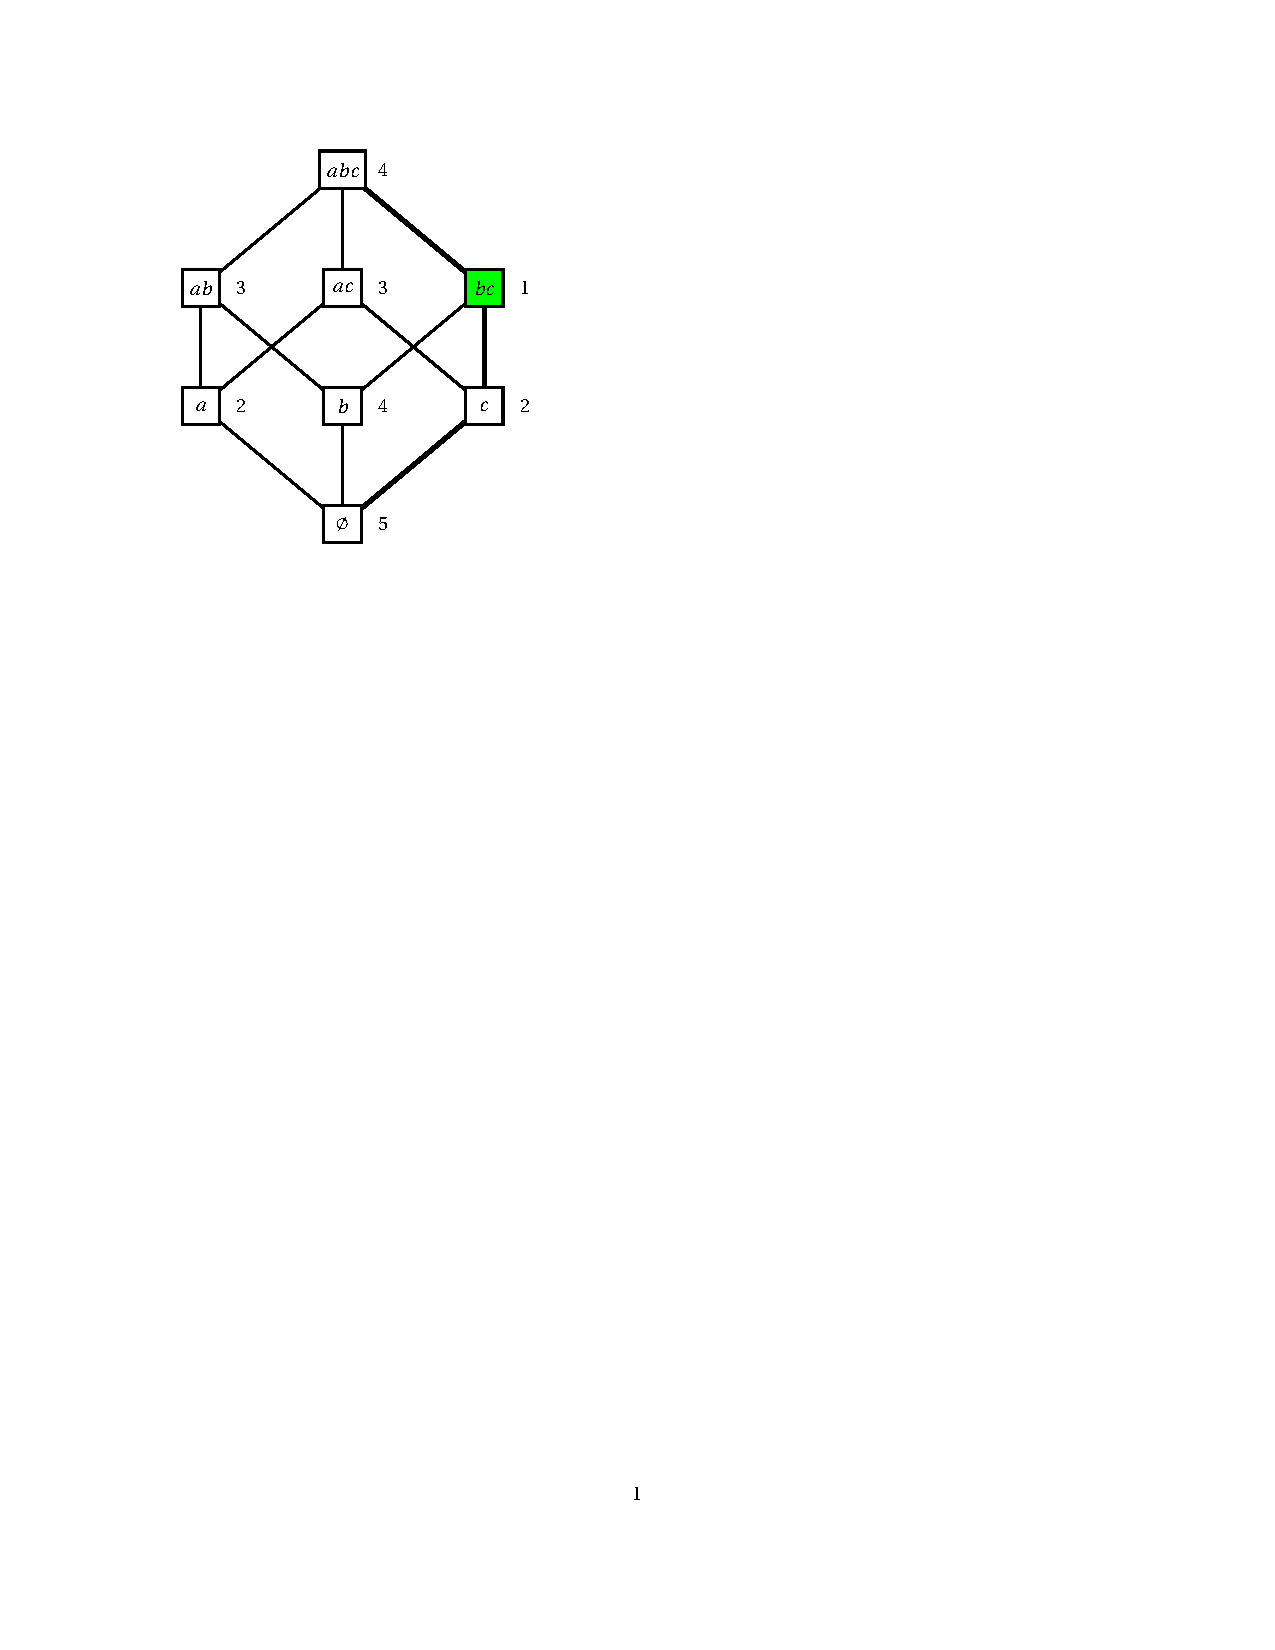
\includegraphics[width=.2\textwidth,clip=true, trim={3cm 18cm 13cm 2cm}]{example_lattice_3.pdf}
    %} & \phantom{abcdefgh} &
    %\subfigure {
        %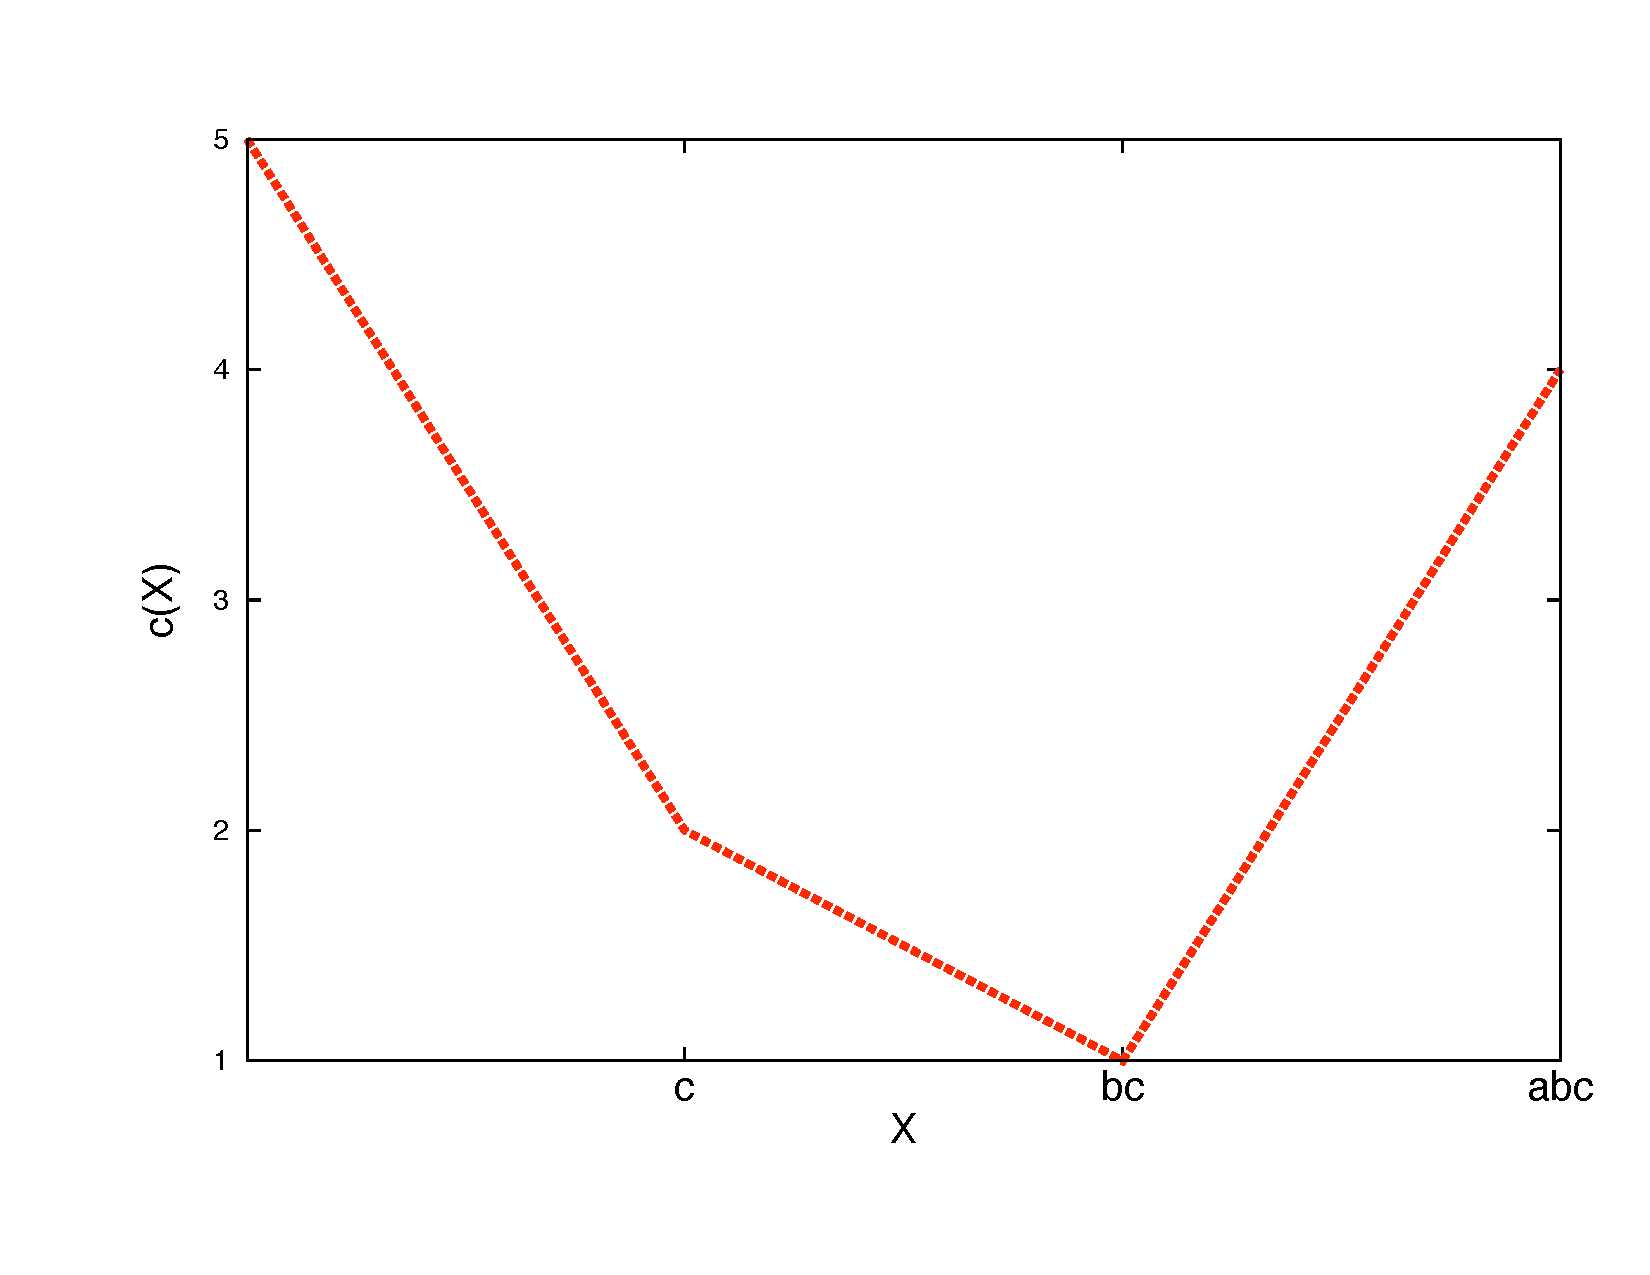
\includegraphics[width=.3\textwidth,clip=true, trim={1cm 0cm 1cm 2cm}]{example_lattice_chain_3.pdf}
    %}
    %\end{tabular}   
    %\captionsetup{width=.95\linewidth}
    %\caption{Exemplo de instância do problema U-curve com 3 características.}
    %\label{fig:ucurve_example}
%\end{figure}
}
\end{block}


%%%%%%%%%%%%%%%%%%%%%%%%%%%%%%%%%%%%%%%%%%%%%%%%%%%%%%%%%%%%%%%%%%%%%%%%                                     
\begin{block}{Algoritmos de florestas}%
\paragraph{
O algoritmo da literatura Poset-Forest-Search (PFS) representa o
espaço de busca com duas florestas (Fig.~\ref{fig:pfs:forests}). A busca 
pelo ótimo se dá pelo percorrimento de cadeias nestas florestas. A 
hipótese U-curve permite que hajam podas durante este percorrimento.}
    
\vspace{-1cm}
\begin{figure}[!ht]
  \centering 
  \begin{tabular}{l c r}
    \subfigure{
        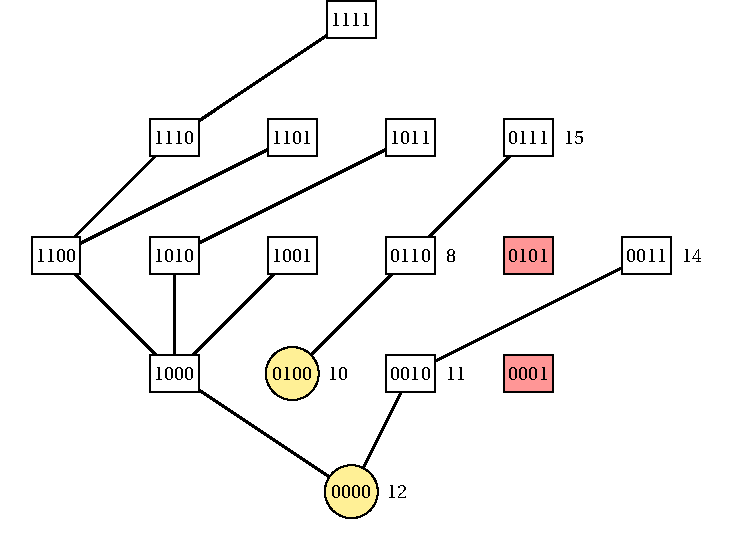
\includegraphics[clip=true, width=.35\textwidth]{pfs/race_cond/raceA.pdf}
    }
    & 
    \phantom{abcdefgh}
    &
    \subfigure{
        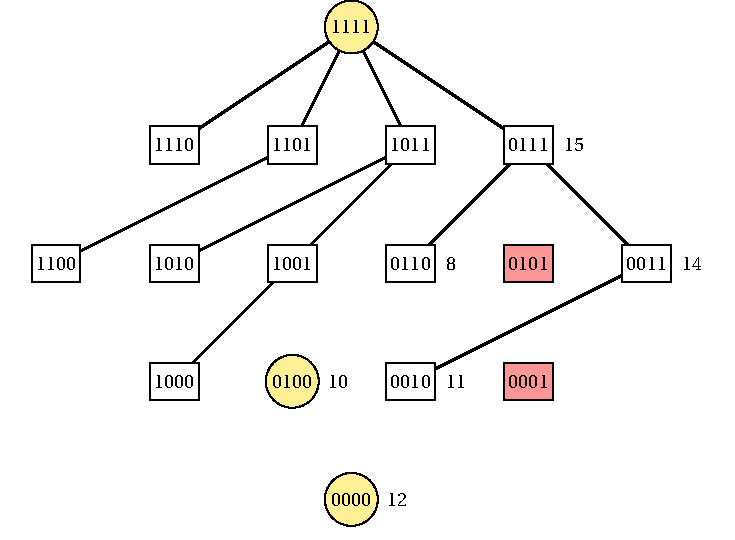
\includegraphics[clip=true, width=.35\textwidth]{pfs/race_cond/raceB.pdf}
    }
  \end{tabular}
  \captionsetup{width=.92\linewidth}
  \centering
  \caption{Exemplo de florestas do algoritmo PFS. Os nós em vermelho
    foram removidos do espaço de busca, enquanto os nós em amarelo
    são raízes da floresta.}
  \label{fig:pfs:forests} 
\end{figure}

\paragraph{Implementamos uma variação do PFS que modifica o 
armazenamento e a escolha de raízes para percorrimentos na floresta, o
ROBDD PFS (RPFS). Também para paralelizamos este algoritmo, criando o
Parallel PFS (PPFS). Além disso, criamos um novo algoritmo paralelo que 
usa o U-Curve-Branch-and-Bound (UBB) para decompor a floresta em 
árvores menores que são resolvidas por chamadas independentes do PFS;
este chamamos de UBB-PFS.}
\end{block}

\vspace{-1cm}
\begin{block}{Parallel-U-Curve-Search}
\paragraph{O Parallel-U-Curve-Search (PUCS) particiona o espaço de busca 
em estruturas que também são reticulados Booleanos. Esta divisão do 
espaço de busca permite aplicações recursivas do algoritmo e a solução
paralela de cada parte. O algoritmo que resolve cada parte é chamado
de algoritmo base.}

\begin{figure}[h]
  \begin{tabular}{l c r}
  \centering
  \subfigure {
    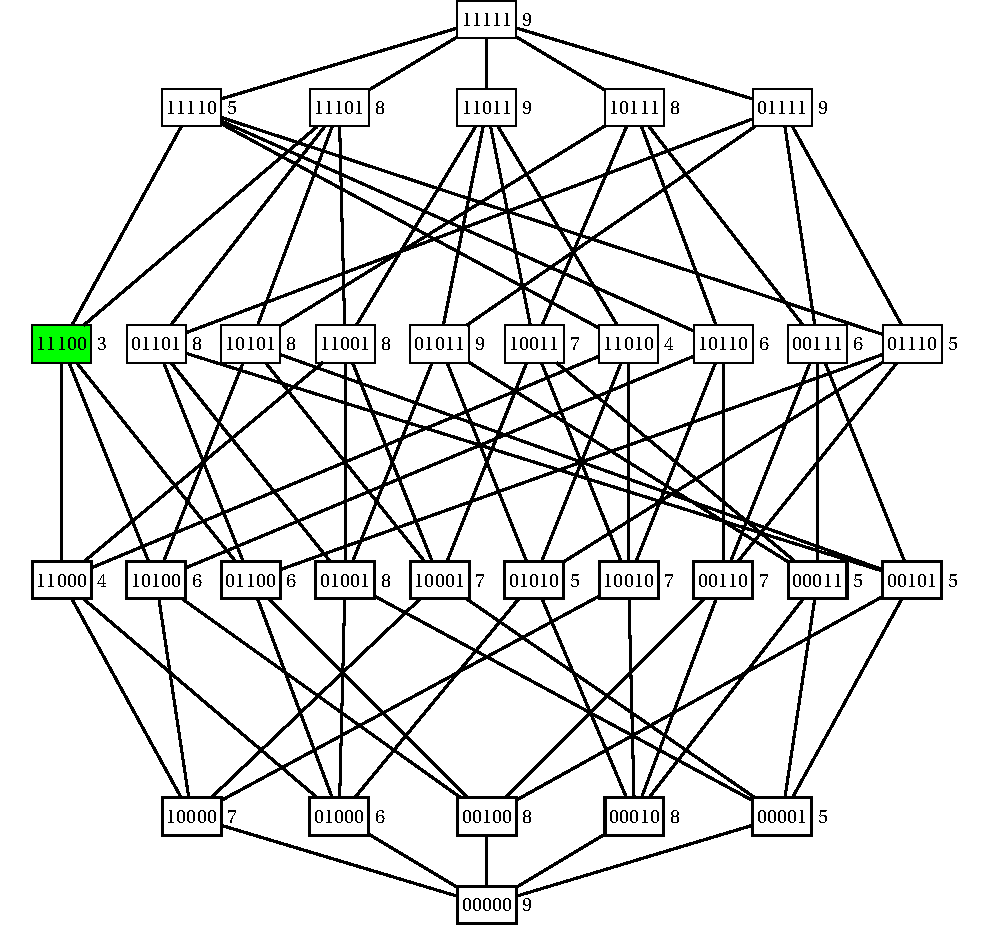
\includegraphics[clip=true, width=0.35\textwidth]{simulation/Boolean_lattice.pdf}
  }
  & \phantom{abcdefgh} &
  \subfigure {
    \label{fig:example:A}
      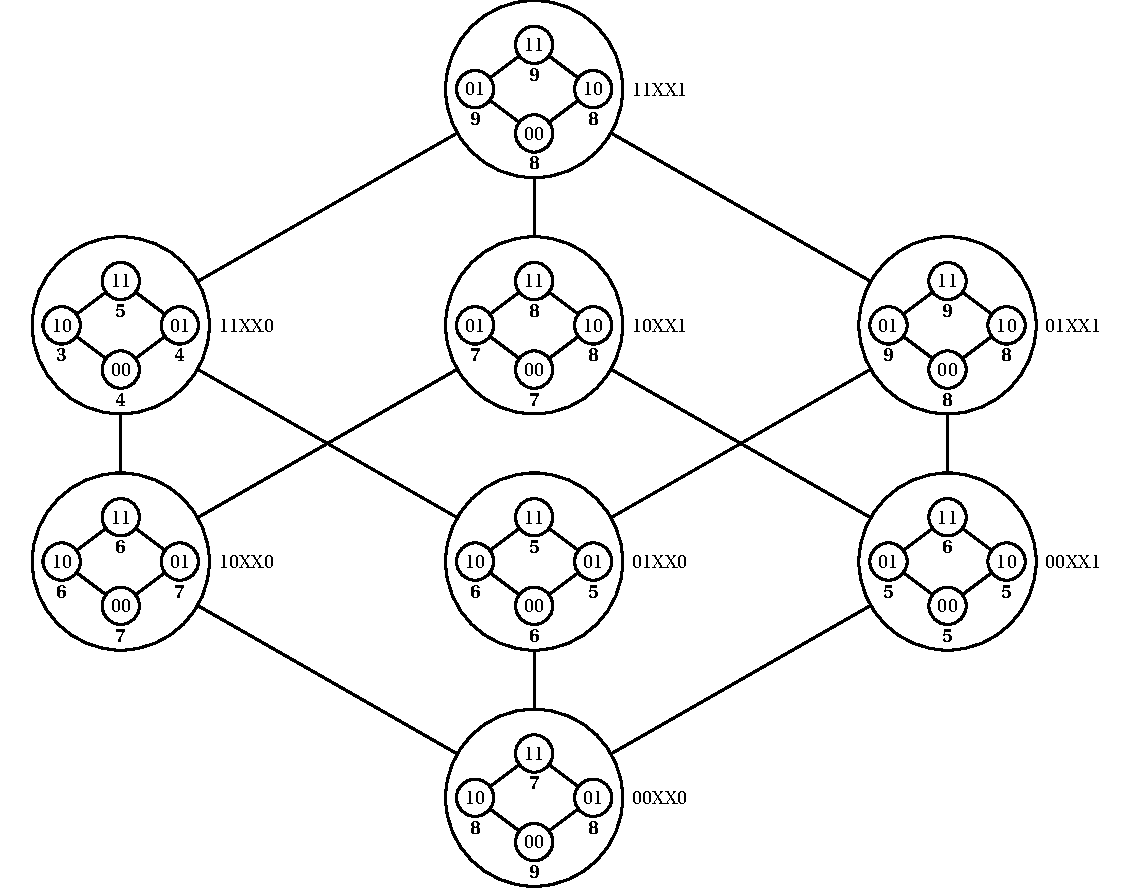
\includegraphics[clip=true, width=0.35\textwidth]{simulation/A.pdf}
  }
  \end{tabular}   
  \captionsetup{width=.92\linewidth}
  \caption{Instância do problema U-curve com $|S| = 5$ (esquerda) e o
    particionamento feito quando a terceira de quarta variável são
    escolhidas como don't cares (direita).}
\end{figure}

\end{block}

\vfill 
\vspace*{.5cm}%
\begin{block}{Apoio Financeiro}%
% \insidecolumns{0.2}{2}%
% {\mycenteredimage{institutions/FAPESP.jpg}{1.1}}%
% {\mycenteredimage{institutions/capes.jpg}{1.2}}%
% {\mycenteredimage{institutions/CNPq.png}{1.5}}%

\vspace*{-1.5cm}%
\begin{figure}[h]
    \begin{tabular*}{0.7\textwidth}{c@{\extracolsep{\fill}}cc}
    \centering
    \subfigure {
        
\includegraphics[clip=true, width=0.2\textwidth]{institutions/FAPESP.jpg}
    }
    &
    \subfigure {
        
\includegraphics[clip=true, width=0.2\textwidth]{institutions/CNPq.png}
    }
    &
    \subfigure {
        
\includegraphics[clip=true, width=0.1\textwidth]{institutions/capes.jpg}
    }
    \end{tabular*}   
\end{figure}
\vspace*{1.5cm}%
\end{block}%
} % end \leftcolumn




\rightcolumn{              
\begin{block}{Resultados}%
\leftfigparagraph{qrcode_featsel.png}{5}{10}{
Usamos o {\em featsel}
(\href{github.com/msreis/featsel}{github.com/msreis/featsel}), um 
arcabouço em C++, para implementar e avaliar os novos algoritmos,
comparando com soluções da literatura. Os testes foram conduzidos em uma
servidora de 64 cores e 256 GB de memória RAM.
} % paragraph
\vspace{-1.5em}

\begin{figure}[h]
\centering
\begin{tabular}{l c r}
    \centering
    \subfigure {
        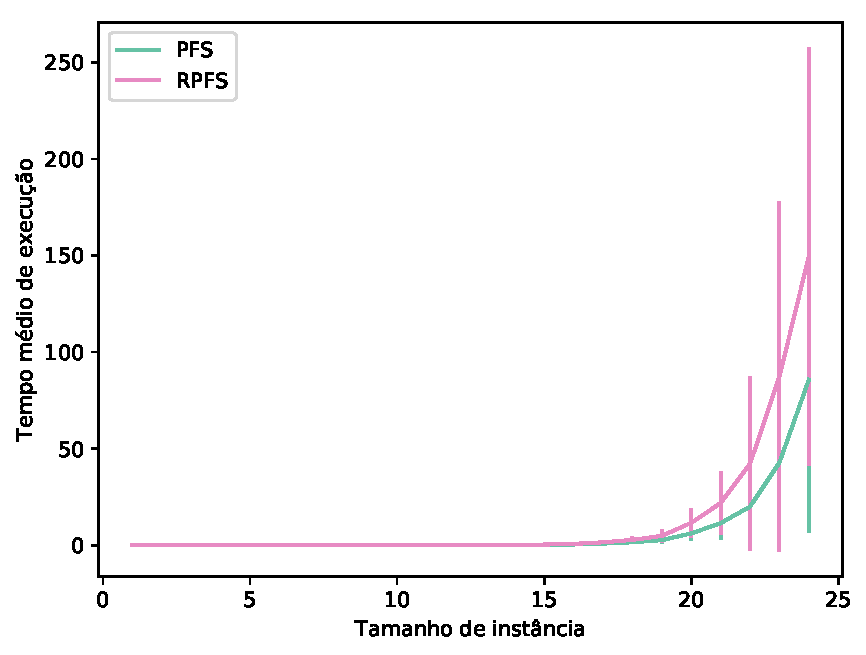
\includegraphics[clip=true, width=0.35\textwidth]{results/rpfs_avg_time.pdf}
    }
    & 
    \phantom{abcdef}
    &
    \subfigure {
        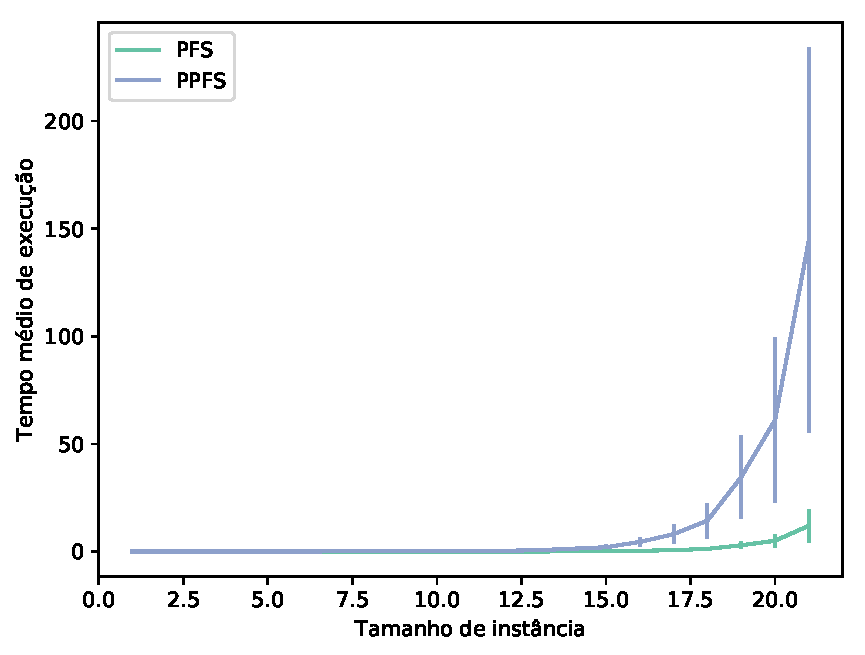
\includegraphics[clip=true, width=0.35\textwidth]{results/ppfs_avg_time.pdf}
    }
\end{tabular}
\captionsetup{width=.92\linewidth}
\caption{Comparação do tempo médio de execução do PFS com as variações
  RPFS e PPFS.}
\label{fig:ppfs_and_rpfs_results}
\end{figure}

\vspace{-1cm}
\begin{figure}[h]
\centering
\begin{tabular}{l c r}
    \centering
    \subfigure {
        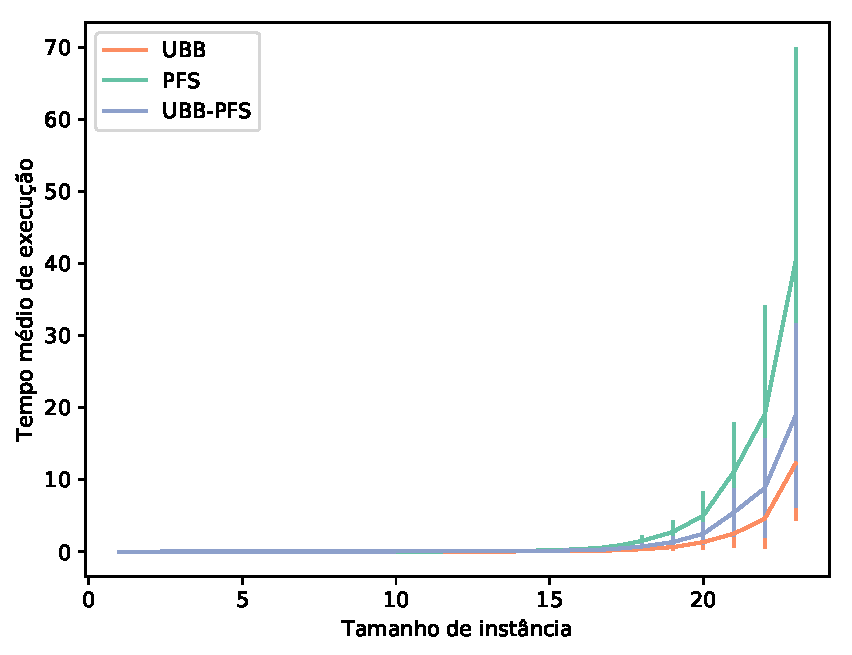
\includegraphics[clip=true, width=0.35\textwidth]{results/ubb-pfs_avg_time.pdf}
    }
    & 
    \phantom{abcdef}
    &
    \subfigure {
        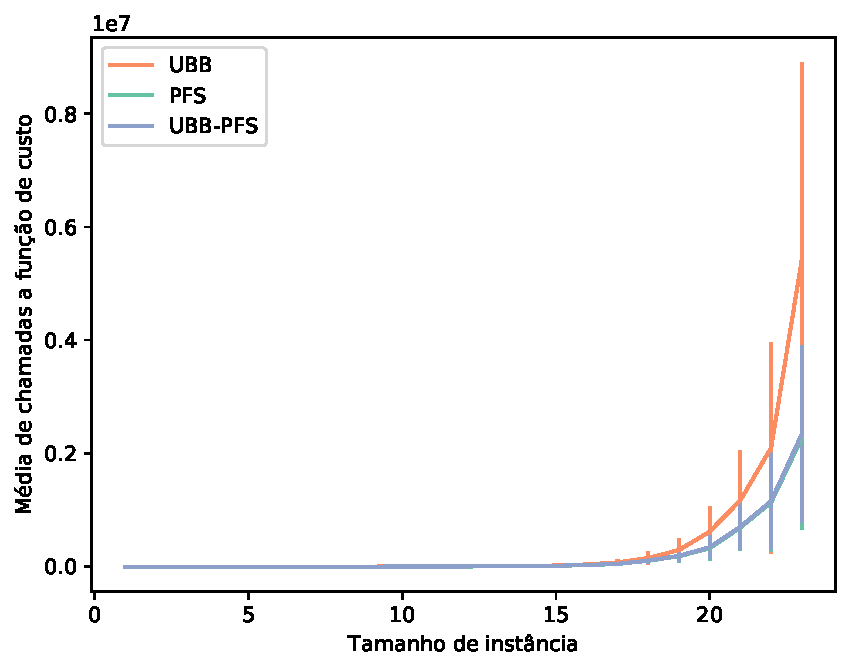
\includegraphics[clip=true, width=0.35\textwidth]{results/ubb-pfs_avg_calls.pdf}
    }
\end{tabular}
\captionsetup{width=.92\linewidth}
\caption{Comparação do tempo médio de execução (esquerda) e número médio
    de chamadas da função custo (direita) feitas pelo UBB-PFS, 
    comparando com o UBB e PFS.}
\label{fig:ubbpfs_results}
\end{figure}


\rightfigparagraph{figures/aproximation_like.png}{12}{6}{%
O algoritmo PUCS possui dois parâmetros, $p$ e $l$ que definem a 
granularidade do particionamento. Quando o algoritmo base é uma 
heurística, notamos que estes parâmetros também controlam a qualidade da
solução obtida pelo PUCS. Comparamos o PUCS heurístico com os algoritmos
Sequential Forward Floating Selection (SFFS) e Best-First Search (BFS).
}%

\vspace{-1.5em}

\begin{figure}[h]
    \begin{tabular}{l c r}
    \centering
    \subfigure {
        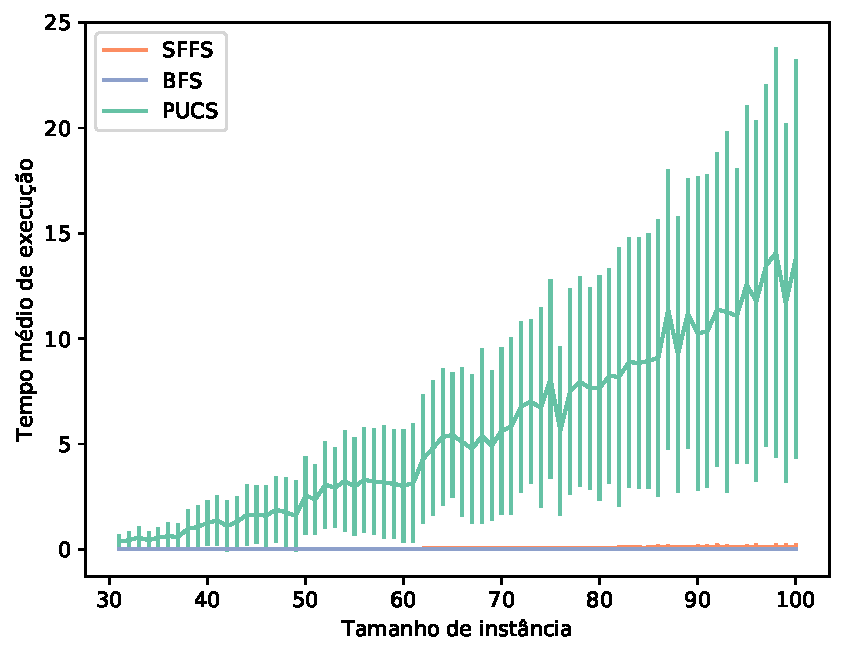
\includegraphics[clip=true, width=0.35\textwidth]{results/pucs_avg_time.pdf}
    }
    &
    \phantom{abcdef}
    &
    \subfigure {
        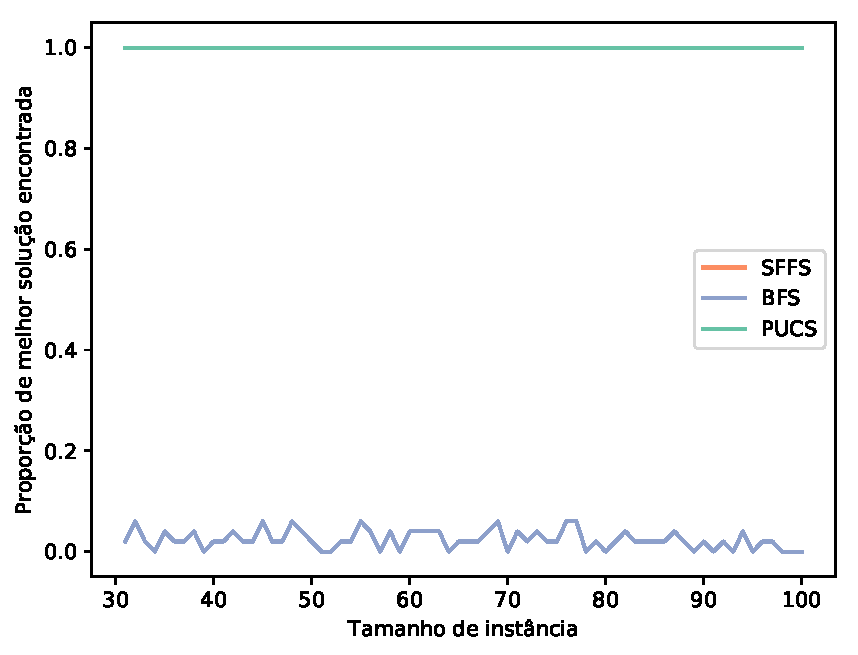
\includegraphics[clip=true, width=0.35\textwidth]{results/pucs_correctness.pdf}
    }
    \end{tabular}   
    \captionsetup{width=.92\linewidth}
    \caption{Tempo de execução e proporção de melhor resposta encontrada
        pelos algoritmos sub-ótimos PUCS, SFFS e BFS.}
\end{figure}

\begin{figure}[h]
\centering
\begin{tabular}{l c r}
    \centering
    \subfigure {
        \label{fig:art_res:small:time}
        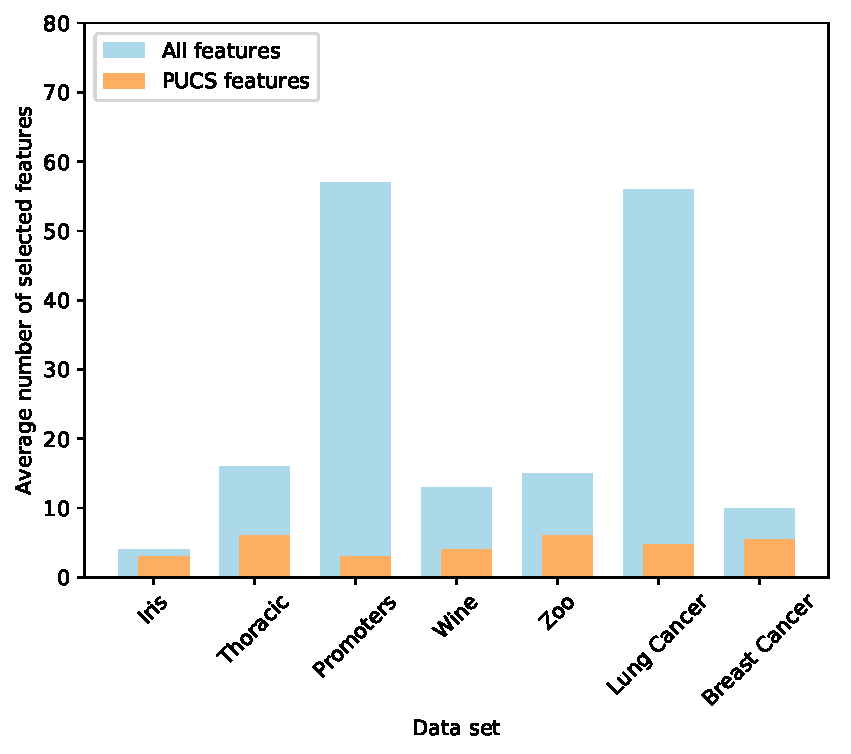
\includegraphics[clip=true, width=0.35\textwidth]{results/avg_features.pdf}
    }
    &
    \phantom{abcdef}
    &
    \subfigure {
        \label{fig:art_res:small:correctness}
        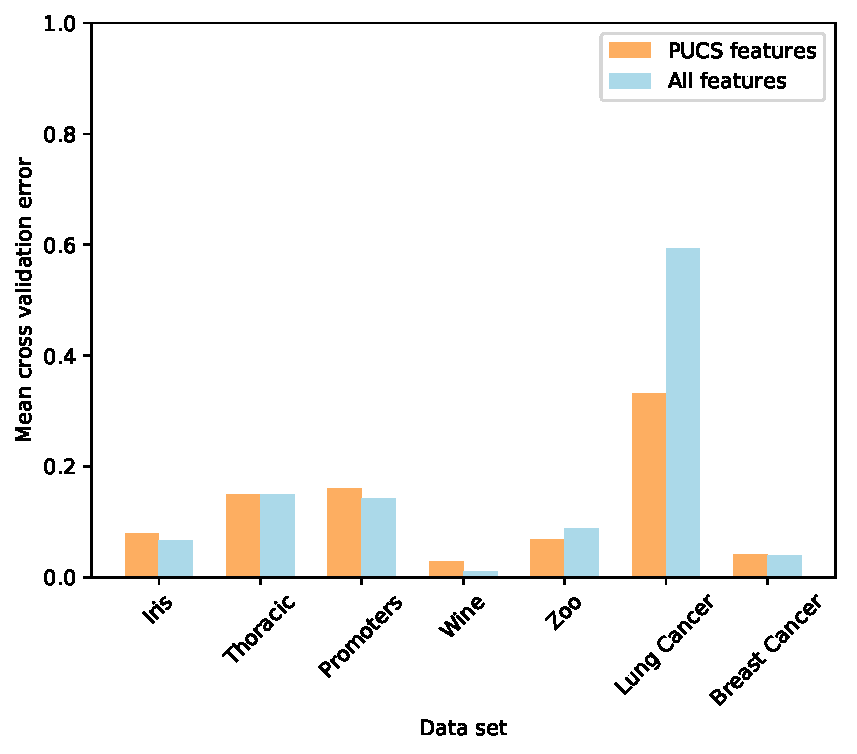
\includegraphics[clip=true, width=0.35\textwidth]{results/svm_error.pdf}
    }
\end{tabular}
\captionsetup{width=.95\linewidth}
\caption{Número médio de características selecionadas pelo PUCS e erro 
    médio de validação cruzada quando utiliza-se as características 
    selecionadas no projeto de classificadores do tipo SVM. Estes 
    conjuntos de dados foram extraídos do UCI Machine Learning 
    Repository.}
\label{fig:svm_error}
\end{figure}

\end{block}



%%%%%%%%%%%%%%%%%%%%%%%%%%%%%%%%%%%%%%%%%%%%%%%%%%%%%%%%%%%%%%%%%%%
\begin{block}{Conclusão}%
\paragraph{
Neste trabalho fomos capazes de criar algoritmos competitivos para o
problema U-Curve e também confirmamos a eficácia da seleção de 
característiacs na seleção de modelos de aprendizado. Trabalhos futuros
nesta linha incluem:
    \begin{itemize}
        \item{Avaliação de robustez dos novos algoritmos quando a hipótese
            U-curve tem violações.}
        \item{Aplicação de seleção de características na identificação
            de vias de sinalização celular}
    \end{itemize}
}
\end{block}
}% end of right column
\end{columns}
\end{frame}
\end{document}
